\documentclass[./../main_file.tex]{subfiles}
\begin{document}
	Là mô tả về góc nhìn ca sử dụng của kiến trúc phần mềm. Khung nhìn ca sử dụng là một dữ liệu đầu
	vào quan trọng cho việc lựa chọn tập các kịch bản và/hoặc các ca sử dụng. Nó mô tả tập các ca kịch 
	bản và/hoặc các ca sử dụng đại diện cho một số chức năng quan trọng. Nó cũng mô tả tập các kịch
	bản và/hoặc các ca sử dụng có phạm vi kiến trúc đáng kể (thực hiện nhiều yếu tố kiến trúc)
	hoặc được nhấn mạnh hay là một minh hoạt cụ thể của kiến trúc.
	
	
	Các ca sử dụng trong hệ thống này được liệt kê dưới đây. Các ca sử dụng được \textbf{in đậm} là 
	các ca sử dụng quan trọng đối với kiến trúc. Mỗi mô tả về các ca sử dụng này sẽ đựợc trình bày 
	sau trong phần này.
	\begin{itemize}
		\item Đăng nhập
		\item Quản lý thông tin cá nhân
		\item \textbf{Tương tác người dùng khác}
		\item Khám phá
		\item Xem giới thiệu
		\item Tìm kiếm lớp học
		\item \textbf{Tham gia lớp học}
		\item Tham gia thảo luận
		\item \textbf{Kiểm tra trực tuyến}
		\item \textbf{Nộp bài tập}
		\item Khám phá lớp học
		\item Phản hồi
		\item Quản lý diễn đàn
		\item Quản lý danh sách sinh viên
		\item \textbf{Quản lý hoạt động sinh viên}
		\item \textbf{Quản lý nội dung lớp học}
		\item \textbf{Quản lý danh sách khóa học}
		\item \textbf{Quản lý tài khoản}
	\end{itemize}

	\subsection{Làm rõ ca sử dụng}
	Các mô hình ca sử dụng sau đây mô tả các ca sử dụng của hệ thống.
	\subsubsection{Khách truy cập}
	\begin{figure}[H]
		\centering
		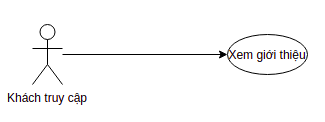
\includegraphics[width=0.6\textwidth]{./images/usecasevisitor.png}
		\caption{Mô hình ca sử dụng của khách truy cập}
	\end{figure}
	\subsubsection{Người dùng}
	\begin{figure}[H]
		\centering
		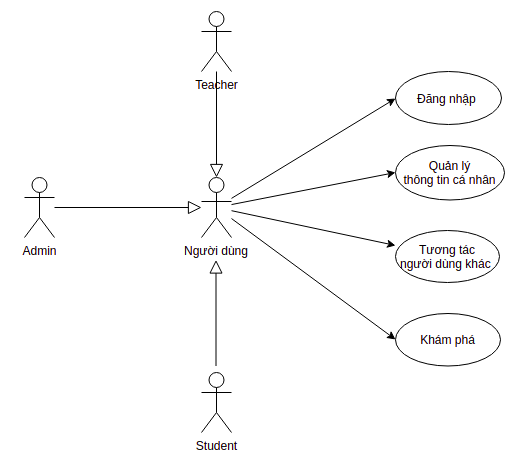
\includegraphics[width=1.0\textwidth]{./images/usecaseuser.png}
		\caption{ Mô hình ca sử dụng của người dùng}
	\end{figure}
	\subsubsection{Sinh viên}
	\begin{figure}[H]
		\centering
		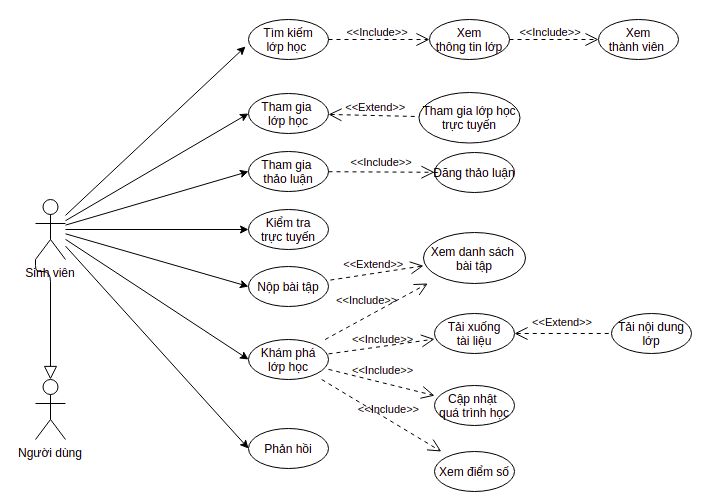
\includegraphics[width=\textwidth]{./images/usecasestudent.png}
		\caption{Mô hình ca sử dụng của sinh viên}
	\end{figure}
	\subsubsection{Giảng viên}
	\begin{figure}[H]
		\centering
		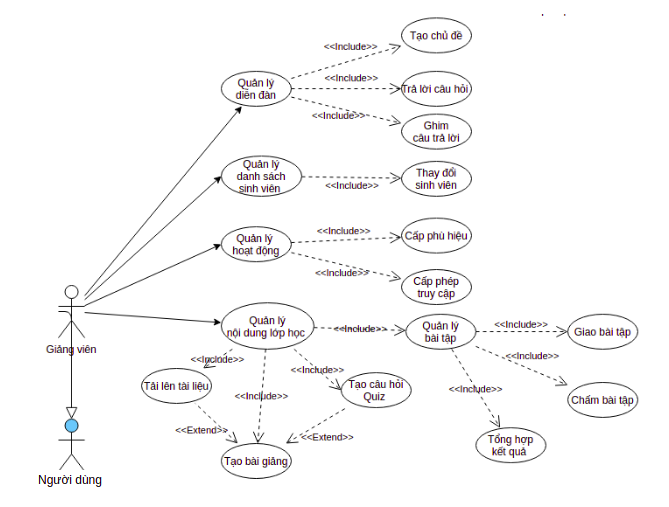
\includegraphics[width=\textwidth]{./images/usecaseteacher.png}
		\caption{Mô hình ca sử dụng của giảng viên}
	\end{figure}
	\subsection{Mô tả ca sử dụng tiêu biểu}
	\begin{description}
		\item[Tương tác người dùng khác] Hệ thống có các tác vụ như đăng blog, nhắn tin thảo luận giữa những người dùng trong cùng một khóa học. Người dùng có thể xóa tin nhắn, xóa cuộc trò chuyện ở phía mình.
		\item[Tham gia lớp học] Sinh viên truy cập khóa học để học tập và tham gia các phiên học trực tuyến.
		\item[Kiểm tra trực tuyến] Sinh viên làm bài kiểm tra do giảng viên tạo trên hệ thống trong một khoảng thời gian và số lần truy cập được chỉ định sẵn. Có thể nộp bài trước khi kết thúc thời gian và bài được tự động nộp lên hệ thống khi thời gian làm bài kết thúc.
		\item[Nộp bài tập] Sinh viên thực hiện làm bài tập được giao và có thể nộp lên hệ thống với nhiều định dạng (pdf, ảnh, docx,...). Nếu có thời hạn thì sinh viên phải nộp trước thời gian đó.
		\item[Quản lý hoạt động sinh viên] Giảng viên trong khóa học có thể cấp phép truy cập cho sinh viên nếu có yêu cầu, theo dõi quá trình học của sinh viên và cấp huy hiệu cho sinh viên có đóng góp tích cực.
		\item[Quản lý nội dung lớp học] Giảng viên quản lý nội dung được chia sẻ trong khóa học phần. Giảng viên có thể thêm, xóa và sửa tài liệu; hiển thị hoặc ẩn tài liệu có sẵn; di chuyển vị trí tài liệu.
		\item[Quản lý danh sách khóa học] Danh sách các khóa học phần được quản trị viên tạo ra từ các dữ liệu của trường. Quản trị viên có thể kiểm soát, thêm mới, sửa đổi hoặc xóa các khóa học của học kỳ.
		\item[Quản lý tài khoản] Quản trị viên có quyền cấp phát tài khoản sinh viên và giảng viên trong trường, lấy danh sách tài khoản.
		
	\end{description}
\end{document}